\section{Results and Analysis}
\label{sec:results}
\subsection{The first failure can conceal the main remaining obstacle}
\label{sec:phase3results}
The diagnostic framework answers 27/100 GPQA questions and 57/100 murder mysteries correctly without corrections. The 73 GPQA failures are all first diagnosed at retrieval. The 43 murder-mystery failures begin at retrieval in 19 cases, mapping in 3, and adaptation in 21; none begins at schema induction. These are first-failure assignments within unsuccessful workflows, not unconditional stage error rates.

A first-failure label alone suggests that GPQA needs better sources and murder mysteries need better target application. Cumulative repair tests what this account leaves out. After retrieval correction, the same base model solves 17 of the 73 GPQA failures (23.29\%). Mapping correction does not add rescues, and schema correction adds one, bringing the total to 18/73 (24.66\%). For murder mysteries, the cumulative totals are 11, 14, and 15 of 43 failures after retrieval, mapping, and schema correction (25.58\%, 32.56\%, and 34.88\%). Figure~\ref{fig:repairs} follows the same initial failure cohorts.

\begin{figure}[t]
\centering
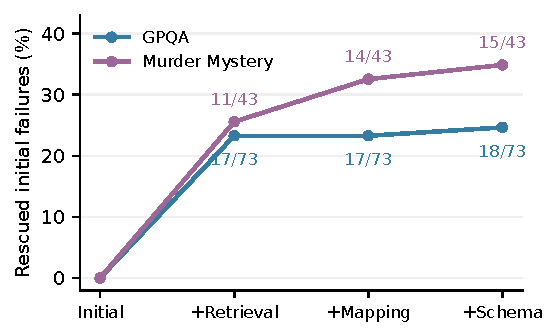
\includegraphics[width=\columnwidth]{figures/phase3_repairs.pdf}
\caption{Cumulative rescue of initially failed workflows after upstream corrections. Counts use the actual cohorts: 73 GPQA and 43 murder-mystery failures. Final gold adaptation is excluded because it supplies the answer rather than testing downstream base-model continuation.}
\label{fig:repairs}
\end{figure}

\paragraph{Failure migration and overlapping burden.}
After upstream corrections, adaptation remains inadequate for 55/73 GPQA failures (75.34\%) and 28/43 murder mysteries (65.12\%). GPQA also reveals mapping problems in 26/73 and schema problems in 15/73 over the correction history; murder mysteries reveal mapping problems in 6/43 and schema problems in 1/43. These burdens overlap because one trajectory can need several repairs. Appendix~\ref{app:states} separates mutually exclusive current states from overlapping cumulative burdens.

The distinction changes the interpretation of the initial diagnosis. Retrieval is the first barrier for every failed GPQA trajectory, but it is not the only barrier: most paths still fail after upstream guidance is corrected. In particular, moving a failure from retrieval to adaptation does not by itself indicate that the retrieval correction damaged the path. It can expose an operation that the original path never reached with an adequate input. Likewise, mapping correction can remove a visible deficiency without increasing final accuracy, because the schema or adaptation remains inadequate.

\paragraph{Rescue requires base-model continuation.}
Natural successes plus genuine continuation after upstream corrections give 45/100 correct GPQA answers and 72/100 correct murder mysteries. These are assisted workflow outcomes. Replacing adaptation with a reference-informed final answer is excluded: that intervention supplies the result instead of testing the solver's ability to finish. Reporting it as model rescue would erase precisely the downstream difficulty that the framework identifies.

The domain contrast is compatible with the task demands. Scientific questions require external knowledge to understand the target and obtain useful sources. Murder mysteries provide many relevant facts but require instantiating relations under particular story constraints. These results do not identify hidden mechanisms; they show why observable source adequacy and target adaptation need separate assessment.

\subsection{Solved sources can support structure-dependent transfer}
\label{sec:phase2results}
To establish that sources can help through more than their mere presence, we examine the factorial source-answer test in Table~\ref{tab:phase2}. Llama-1B gains 5.50 points when either the corresponding or random source answer is provided, yielding zero mean interaction. Llama-3B gains about 13.92 points from corresponding source content in both answer settings, but the answer adds the same 2.91 points in either source type. Its zero interaction therefore does not mean the corresponding source is useless; it means the observed answer benefit is not selective.

\begin{table*}[t]
\centering
\small
\begin{tabular}{@{}lrrrrr@{}}
\toprule
Model & $A$: true/no answer & $B$: true/answer & $C$: random/no answer & $D$: random/answer & $\Delta_{\mathrm{transfer}}$ \\
\midrule
Llama-3.2-1B & $38.51\pm1.48$ & $44.01\pm0.56$ & $38.51\pm2.02$ & $44.01\pm0.56$ & $0.00$ \\
Llama-3.2-3B & $54.05\pm1.48$ & $56.96\pm0.56$ & $40.13\pm1.12$ & $43.04\pm1.48$ & $0.00$ \\
Llama-3.1-8B & $52.10\pm3.68$ & $65.70\pm3.41$ & $52.43\pm1.94$ & $51.78\pm7.35$ & $+14.24$ \\
Llama-3.1-70B & $59.22\pm3.88$ & $72.17\pm8.76$ & $53.07\pm2.24$ & $53.07\pm2.02$ & $+12.94$ \\
\midrule
Qwen3-14B & $66.02\pm4.12$ & $75.24\pm0.69$ & $60.68\pm2.06$ & $60.68\pm3.43$ & $+9.22$ \\
Qwen3-32B & $68.93\pm2.75$ & $74.27\pm0.69$ & $65.53\pm2.06$ & $58.25\pm2.75$ & $+12.62$ \\
\bottomrule
\end{tabular}
\caption{Factorial transfer accuracy (\%, mean $\pm$ run SD) on the same 103 MuSR targets in every cell. Llama has three runs; Qwen has two. Interactions are in percentage points, computed from unrounded run-level values; rounding displayed cells can produce small discrepancies. SD is not an inferential confidence interval.}
\label{tab:phase2}
\end{table*}

Llama-8B and 70B show a different pattern. The 8B model gains 13.59 points from the corresponding answer and changes by $-0.65$ points with the random answer, giving a 14.24-point interaction. The 70B model gains 12.94 points from the corresponding answer and none from the random answer. These results support structure-dependent use of source answers under the tested protocol. They do not show that every correct answer used the source or that transfer grows monotonically with model size.

The pattern also appears outside the Llama family. Qwen-14B gains 9.22 points from the corresponding answer, with no change in the random-answer mean. Qwen-32B combines a 5.34-point corresponding-answer gain with a 7.28-point random-answer loss, giving a 12.62-point interaction. Its larger interaction does not mean a larger benefit from the valid guide: part of the difference comes from damage in the control. The individual cells are essential to the interpretation.

\paragraph{Transferring an answer role is different from copying an index.}
Llama-1B achieves 88.24\% accuracy when source and target correct-answer positions match and only 0.64\% when they differ. Together with equal answer gains for corresponding and random sources, this suggests predominant index following. Llama-8B and 70B retain 57.05\% and 65.38\% accuracy in the different-position stratum, compared with 74.51\% and 79.08\% in the matching stratum. Their performance is compatible with more than index copying, although position sensitivity persists. Since the strata contain different questions, this check supports rather than independently establishes the factorial interpretation.

Thus, there is positive evidence for selective source use in several evaluated models, alongside substantially different behaviors in smaller models. The framework is useful in this setting because a capacity demonstrated under a supplied source does not guarantee that a model can obtain, abstract, and apply an adequate source on its own.

\subsection{Aggregate gains and textual mention are insufficient measures}
\label{sec:phase1results}
The scientific controls explain why the stronger attribution test and stage diagnosis are needed. In Table~\ref{tab:phase1}, the concept-focused 300-word analogy does not outperform both random controls for any solver. Llama performs slightly better with a same-domain random source, Qwen matches it, and Mistral trails both random controls. Gemma lies between its controls, with the additional caveat of differing retained sets. The intended example relation does not yield a general advantage in final accuracy.

\begin{table*}[t]
\centering
\small
\begin{tabular}{@{}lrrrr@{}}
\toprule
Condition & Llama-8B & Qwen-8B & Mistral-7B & Gemma-31B \\
\midrule
Analogy, 300 words & 30.80 & 36.61 & 27.01 & 65.39 \\
Analogy, 600 words & 31.25 & 36.83 & 28.79 & 68.69 \\
Two analogies, $2\times300$ words & 31.92 & 35.27 & 30.58 & 69.00 \\
Three analogies, $3\times200$ words & 31.03 & 39.73 & 26.56 & 69.61 \\
Non-analogical explanation, 300 words & 31.03 & 37.72 & 27.68 & 68.25 \\
Non-analogical explanation, 600 words & 30.58 & 36.61 & 25.89 & 68.47 \\
Random same-domain analogy, 300 words & 31.25 & 36.61 & 27.68 & 64.85 \\
Random different-domain analogy, 300 words & 29.69 & 39.73 & 28.13 & 67.12 \\
Chain-of-thought & 32.14 & 42.19 & 16.96 & 66.52 \\
Self-analogy & 28.79 & 43.30 & 22.54 & 64.06 \\
\bottomrule
\end{tabular}
\caption{Scientific question-answering accuracy (\%) on GPQA Main. Llama, Qwen, and Mistral have 448 retained responses per condition. Gemma has 435--447, so its overall contrasts can also reflect changes in the retained question set. Recorded responses without a final answer are incorrect.}
\label{tab:phase1}
\end{table*}

\paragraph{The comparison determines the claim.}
Mistral's teacher analogy raises accuracy from 16.96\% under CoT to 27.01\%. Yet a 300-word non-analogical explanation reaches 27.68\%. A gain against CoT therefore does not establish a benefit requiring analogical presentation. Llama's teacher analogy and explanation both trail its CoT baseline. Qwen's self-analogy reaches 43.30\%, compared with 42.19\% for CoT and 36.61\% for the teacher analogy. These are effects of particular assistance and prompting conditions, not interchangeable measures of transfer.

Longer or more numerous examples also fail to provide a uniform benefit. Doubling analogy length adds 0.45 points for Llama and 0.22 for Qwen. At a nominal total of 600 words, Mistral's one-, two-, and three-example accuracies are 28.79\%, 30.58\%, and 26.56\%, while explicit mentions increase from 12.05\% to 19.42\% and 29.24\%. Increased engagement with examples in the output is not direct evidence that a usable schema was induced.

\paragraph{Net improvement can coexist with damage.}
On the same 448 items, Mistral's 300-word analogy repairs 86 CoT errors (19.20\% of all items) while making 41 previously correct answers incorrect (9.15\%). The 45-item net gain is 10.04 percentage points. Two 300-word examples repair 105 answers and damage 44. Figure~\ref{fig:transitions} makes both directions visible. These are condition-associated changes: differing instructions and similar changes under random controls prevent assigning every regression to a faulty analogical mapping.

\begin{figure}[t]
\centering
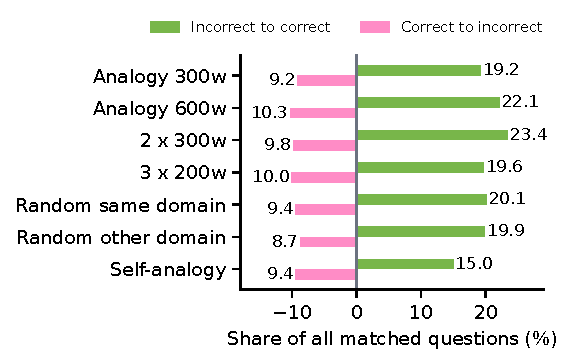
\includegraphics[width=\columnwidth]{figures/phase1_transitions.pdf}
\caption{Mistral transitions relative to CoT on the same 448 questions. Improvements and regressions use all shared items as denominator. Their difference is the net accuracy change.}
\label{fig:transitions}
\end{figure}

\paragraph{Mention is neither successful transfer nor its necessary trace.}
Qwen mentions the 300-word example in 31.70\% of all responses, compared with 8.31\% for Gemma despite Gemma's higher accuracy. Qwen's mention rates within correct and incorrect answers are 31.10\% and 32.04\%. Explicit reference can accompany either outcome, and absence of reference does not prove that the example had no effect. Diagnosing the actual intermediate artifacts gives a more specific question: did the source provide an adequate relation, was it preserved in the schema, and was it applied under the target constraints?

Together, these evaluations establish a hierarchy of evidence rather than a single ranking. Outcome changes show practical effects; controls narrow their attribution; selective source-answer gains support transfer under an intended correspondence; and stage interventions reveal what prevents that process from completing. The claim supported by each measurement depends on the information and operations it actually tests.
